\documentclass[border=3pt]{standalone}
% Shared TikZ styles for the Ch. 3–8 diagrams (standalone PDFs); extends the Ch. 1 palette (s1_vs_llm_common.tex).
\usepackage[T1]{fontenc}
\usepackage{lmodern}
\usepackage[english]{babel}
\usepackage{amsmath,amssymb}
\usepackage{tikz}
\usetikzlibrary{shapes.geometric,shapes.misc,positioning,fit,arrows.meta,calc,backgrounds,decorations.pathreplacing,patterns}
\definecolor{ioFill}{HTML}{F1F0EC}\definecolor{ioLine}{HTML}{52514E}
\definecolor{modFill}{HTML}{E8F1FB}\definecolor{modLine}{HTML}{2A78D6}
\definecolor{decFill}{HTML}{ECE9F7}\definecolor{decLine}{HTML}{4A3AA7}
\definecolor{postFill}{HTML}{FFF6E0}\definecolor{postLine}{HTML}{EDA100}
\definecolor{okFill}{HTML}{EAF7F1}\definecolor{okLine}{HTML}{1BAF7A}
\definecolor{badFill}{HTML}{FDECEC}\definecolor{badLine}{HTML}{E34948}
\definecolor{nmFill}{HTML}{EFEAF8}\definecolor{nmLine}{HTML}{4A3AA7}
\definecolor{loopRed}{HTML}{E34948}\definecolor{clusterLine}{HTML}{9A9890}\definecolor{ink2}{HTML}{52514E}
\definecolor{orangeA}{HTML}{EB6834}
\tikzset{
  every node/.style={font=\small, align=center},
  io/.style={trapezium, trapezium left angle=72, trapezium right angle=108, trapezium stretches body,
             draw=ioLine, fill=ioFill, thick, inner sep=3pt, minimum height=2.4em},
  model/.style={rectangle, draw=modLine, fill=modFill, very thick, inner sep=4pt, minimum height=2.4em, text width=#1},
  model/.default=3.6cm,
  post/.style={rectangle, draw=postLine, fill=postFill, very thick, inner sep=4pt, minimum height=2.2em, text width=#1},
  post/.default=3.6cm,
  data/.style={cylinder, shape border rotate=90, aspect=0.18, draw=okLine, fill=okFill, very thick, inner sep=3pt, minimum height=2.6em, text width=#1},
  data/.default=2.4cm,
  decision/.style={diamond, aspect=2.1, draw=decLine, fill=decFill, very thick, inner sep=1pt},
  outcome/.style={rounded rectangle, draw=#1, thick, inner sep=4pt, minimum height=2em},
  arrow/.style={-{Latex[length=2mm]}, thick, ioLine},
  dashedarrow/.style={-{Latex[length=2mm]}, thick, ioLine, dashed},
  loop/.style={-{Latex[length=2.4mm]}, line width=1.4pt, loopRed},
  cluster/.style={draw=clusterLine, dashed, rounded corners=3pt, inner sep=7pt},
  clusterlabel/.style={font=\small\bfseries, text=ioLine},
  note/.style={font=\footnotesize, text=ink2},
  tok/.style={rectangle, draw=ioLine, fill=ioFill, thin, inner sep=2pt, minimum height=1.6em, font=\footnotesize},
  vmark/.style={rectangle, draw=orangeA, fill=postFill, thick, inner sep=2pt, minimum height=1.6em, font=\footnotesize\ttfamily},
}

\begin{document}
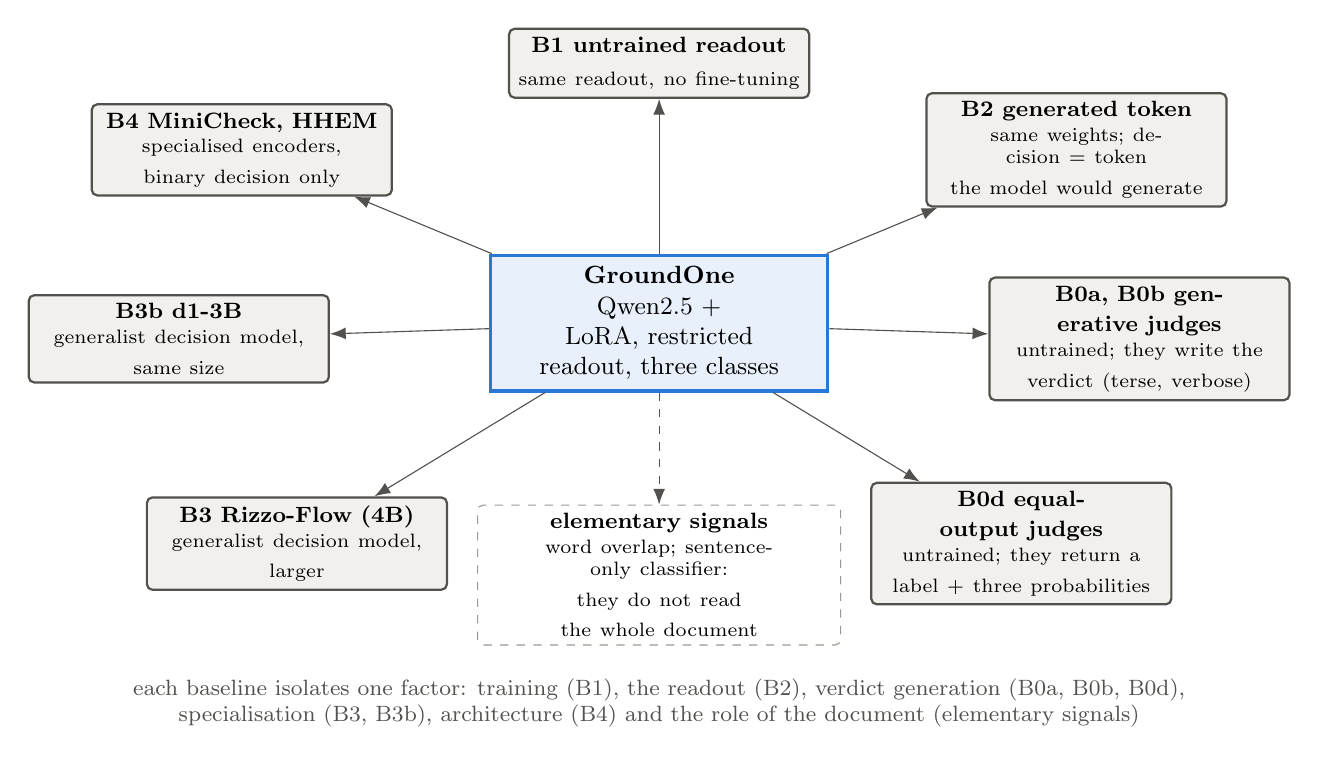
\begin{tikzpicture}
  \node[model=4.0cm, minimum height=1.4cm] (g1) at (0,0) {\textbf{GroundOne}\\Qwen2.5 + LoRA, restricted\\readout, three classes};
  \foreach \pos/\name/\lab/\what in {
      {(0,3.3)}/b1/{B1 untrained readout}/{same readout, no fine-tuning},
      {(5.3,2.2)}/b2/{B2 generated token}/{same weights; decision = token\\the model would generate},
      {(6.1,-0.2)}/b0/{B0a, B0b generative judges}/{untrained; they write the\\verdict (terse, verbose)},
      {(4.6,-2.8)}/b0d/{B0d equal-output judges}/{untrained; they return a\\label + three probabilities},
      {(-4.6,-2.8)}/b3/{B3 Rizzo-Flow (4B)}/{generalist decision model,\\larger},
      {(-6.1,-0.2)}/b3b/{B3b d1-3B}/{generalist decision model,\\same size},
      {(-5.3,2.2)}/b4/{B4 MiniCheck, HHEM}/{specialised encoders,\\binary decision only}} {
    \node[rectangle, rounded corners=2pt, draw=ioLine, fill=ioFill, thick, text width=3.6cm, inner sep=3pt] (\name) at \pos {\textbf{\footnotesize\lab}\\[1pt]{\scriptsize \what}};
    \draw[arrow, thin] (g1) -- (\name);
  }
  \node[rectangle, rounded corners=2pt, draw=clusterLine, dashed, text width=4.4cm, inner sep=3pt] (sig) at (0,-3.2) {\textbf{\footnotesize elementary signals}\\[1pt]{\scriptsize word overlap; sentence-only classifier:\\they do not read the whole document}};
  \draw[dashedarrow, thin] (g1) -- (sig);
  \node[note, below=3mm of sig] {each baseline isolates one factor: training (B1), the readout (B2), verdict generation (B0a, B0b, B0d),\\specialisation (B3, B3b), architecture (B4) and the role of the document (elementary signals)};
\end{tikzpicture}
\end{document}
